\section{Visão computacional}
A visão computacional está em constante avanço, aproximando cada vez mais os computadores da capacidade visual humana. De acordo com Horst Haußecker e Bernd Jähne no livro "Computer Vision and Applications" \cite{comp_vision_and_applications}, a visão computacional é uma área da computação que se dedica à interpretação de imagens por meio de algoritmos e técnicas de processamento de imagens. Essa área abrange a aquisição, processamento e análise de imagens, com o objetivo de extrair informações úteis para resolver problemas específicos.

Porém segundo Richard Szeliski no livro Computer Vision: Algorithms and Applications \cite{computer_vision_richard}, nas ultimas décadas ocorreram avanços significativos na busca de aproximar a visão computacional da visão humana, porem não obteve total êxito. Pois enquanto o olho humano enxerga com aparente facilidade as estruturas tridimensionais e suas nuances, a visão computacional depende de técnicas matemáticas altamente precisas para recuperar a forma tridimensional e a aparência dos objetos.

(podemos ver nas figuras tal e tal que um computador tem a capacidade de distinguir, classificar e até mesmo entender os elementos de uma foto )

No entanto, mesmo com o sucesso no uso dessas técnicas, o computador ainda não é capaz de explicar uma imagem com o mesmo nível de detalhes que o olho humano, pois para um computador é muito mais facil entender o que a gente está falando do que o que a gente está vendo, e explicar pra ele como ver e conseguir descrever com uma riqueza de detalhes aquilo que está vendo é extremamente  complexo.

A visão é um elemento crucial para capacitar a inteligência artificial a realizar diversas tarefas. A fim de replicar a visão humana, é necessário que as máquinas sejam capazes de adquirir, processar, analisar e compreender imagens. \cite{como_funciona_visao_computacional}

Na \cref{fig:comp_vision} podemos ver uma analogia entre a forma como uma imagem é processada pelo cérebro humano e a forma como é processada por um sistema computacional.

\begin{figure}[!ht]
	\centering
	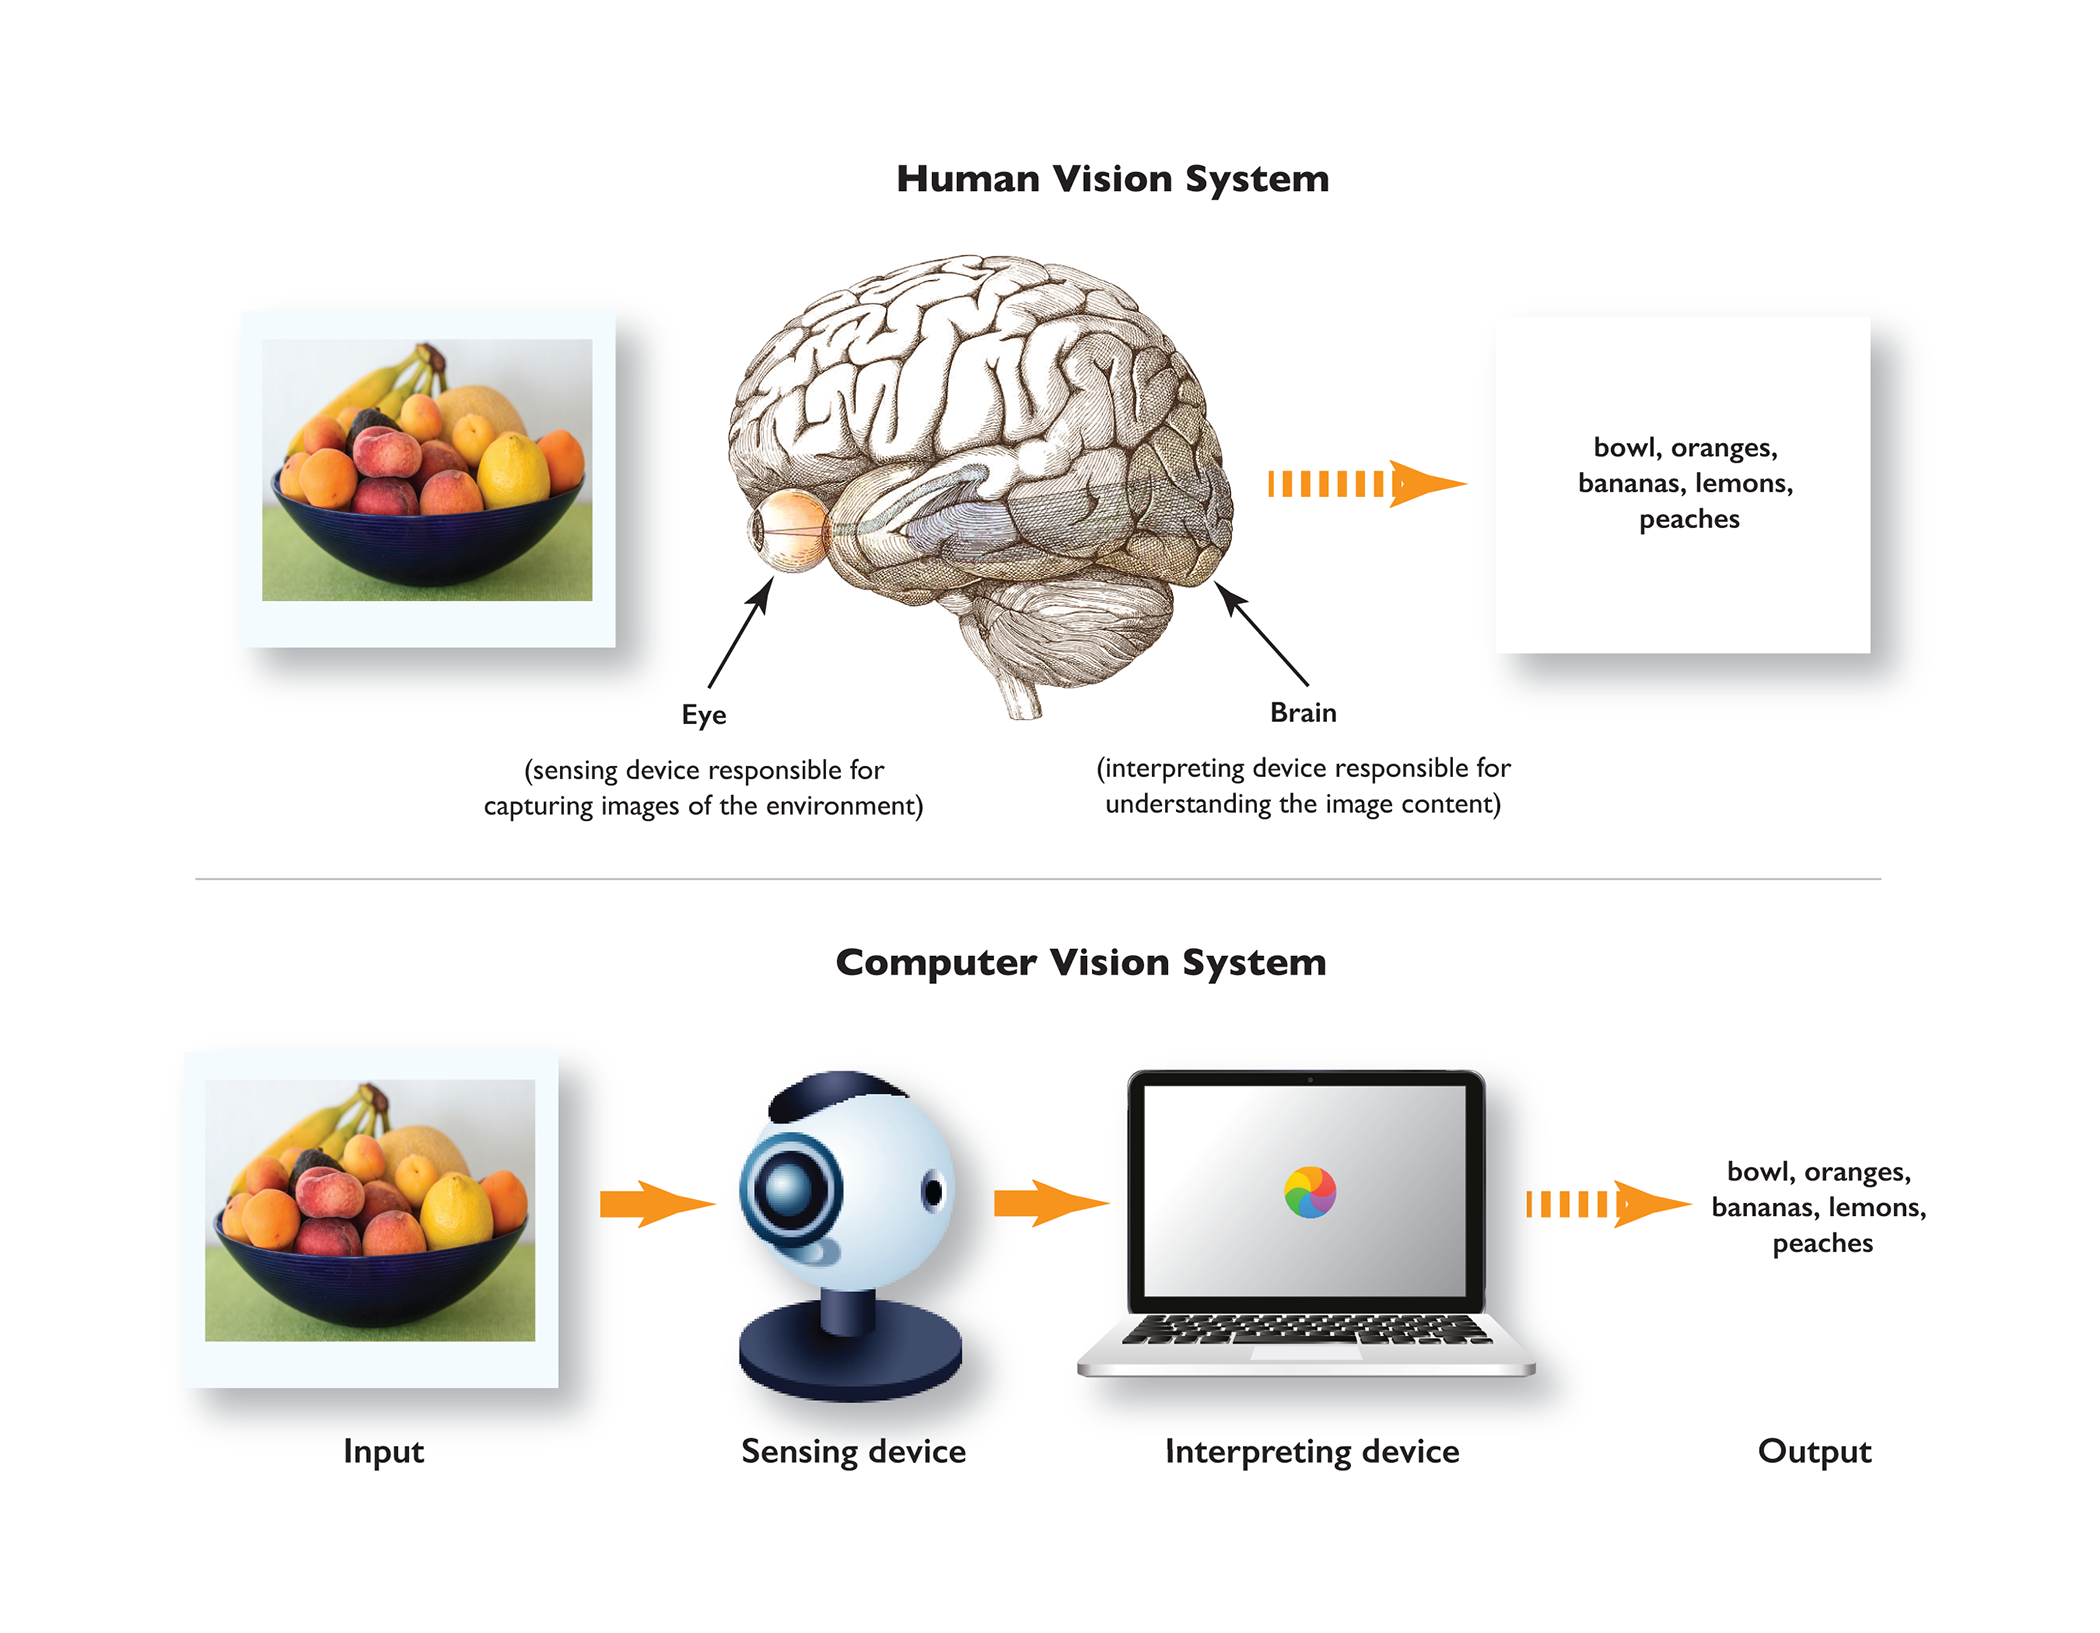
\includegraphics[width=0.6\textwidth]{figures/content_Human_Vision.png}
	\caption{Visão humana e sistemas de visão computacional processam dados visuais de maneira semelhante \cite{content_Human_Vision}.}
	\label{fig:comp_vision}
\end{figure}	

\begin{figure}[!ht]
	\centering
	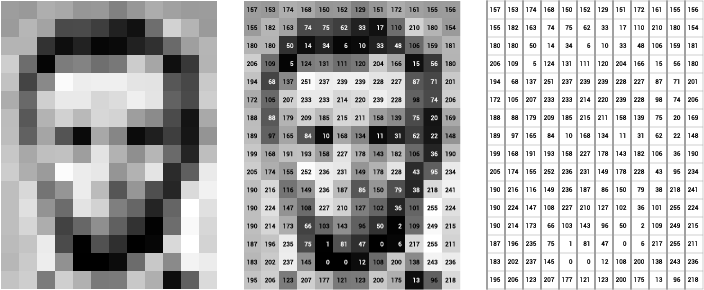
\includegraphics[width=0.6\textwidth]{figures/lincoln_pixel_values.png}
	\caption{Diagrama de dados de pixels. À esquerda, nossa imagem de Lincoln; no centro, os pixels rotulados com números de 0 a 255, representando sua luminosidade; e à direita, apenas esses números \cite{content_Human_Vision}.}
	\label{fig:comp_vision}
\end{figure}

\begin{figure}
    \centering
    \begin{minipage}[b]{0.49\textwidth}
      \centering
      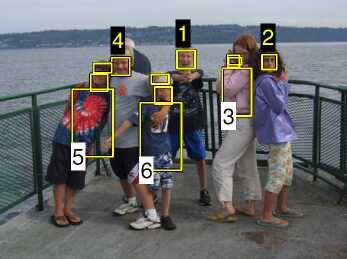
\includegraphics[width=0.6\textwidth]{figures/detectacao_de_faces_exemplo.JPG}
      \caption{Algoritmos de detecção facial e de roupas/cabelos por cor localizam e reconhecem pessoas nesta imagem \cite{computer_vision_richard}}
      \label{fig:imagem_a}
    \end{minipage}
    \hfill
    \begin{minipage}[b]{0.49\textwidth}
      \centering
      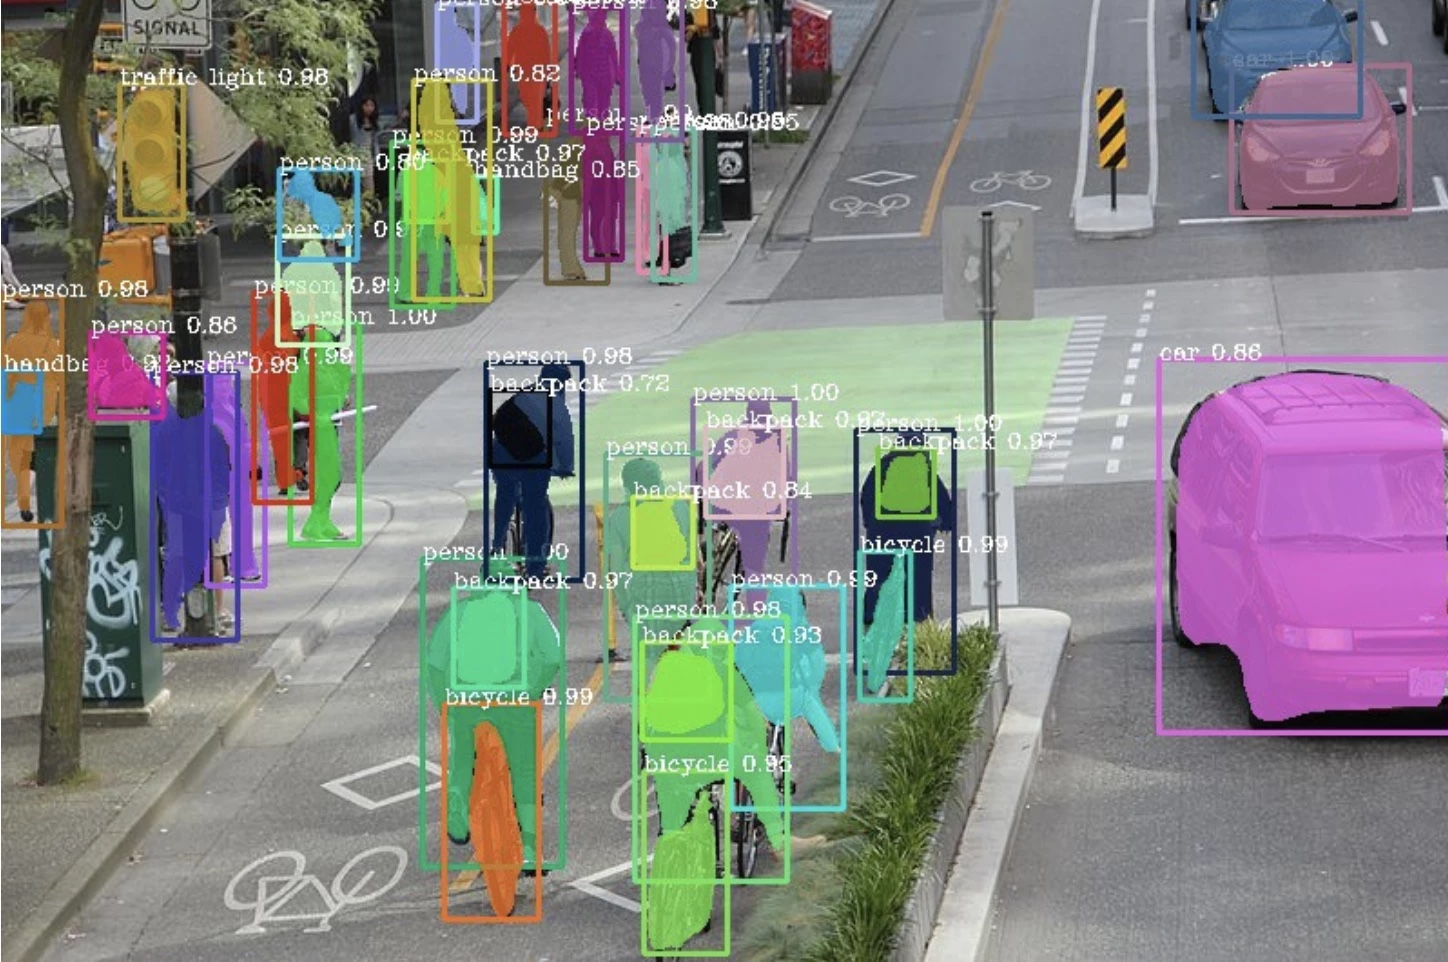
\includegraphics[width=0.6\textwidth]{figures/semantic_intance.JPG}
        \caption{Segmentação de instâncias de objetos pode delinear cada pessoa e objeto em uma cena complexa. 
        \cite{instance_segmentation}}
      \label{fig:imagem_b}
    \end{minipage}
  \end{figure}
  

